\chapter{Results and Discussion}\label{Results}

\blindtext
<during this project, many 

<in the following sections, we will have a look at the 









\section{Data Collection}

\blindtext

\begin{figure}[ht]
\centerline{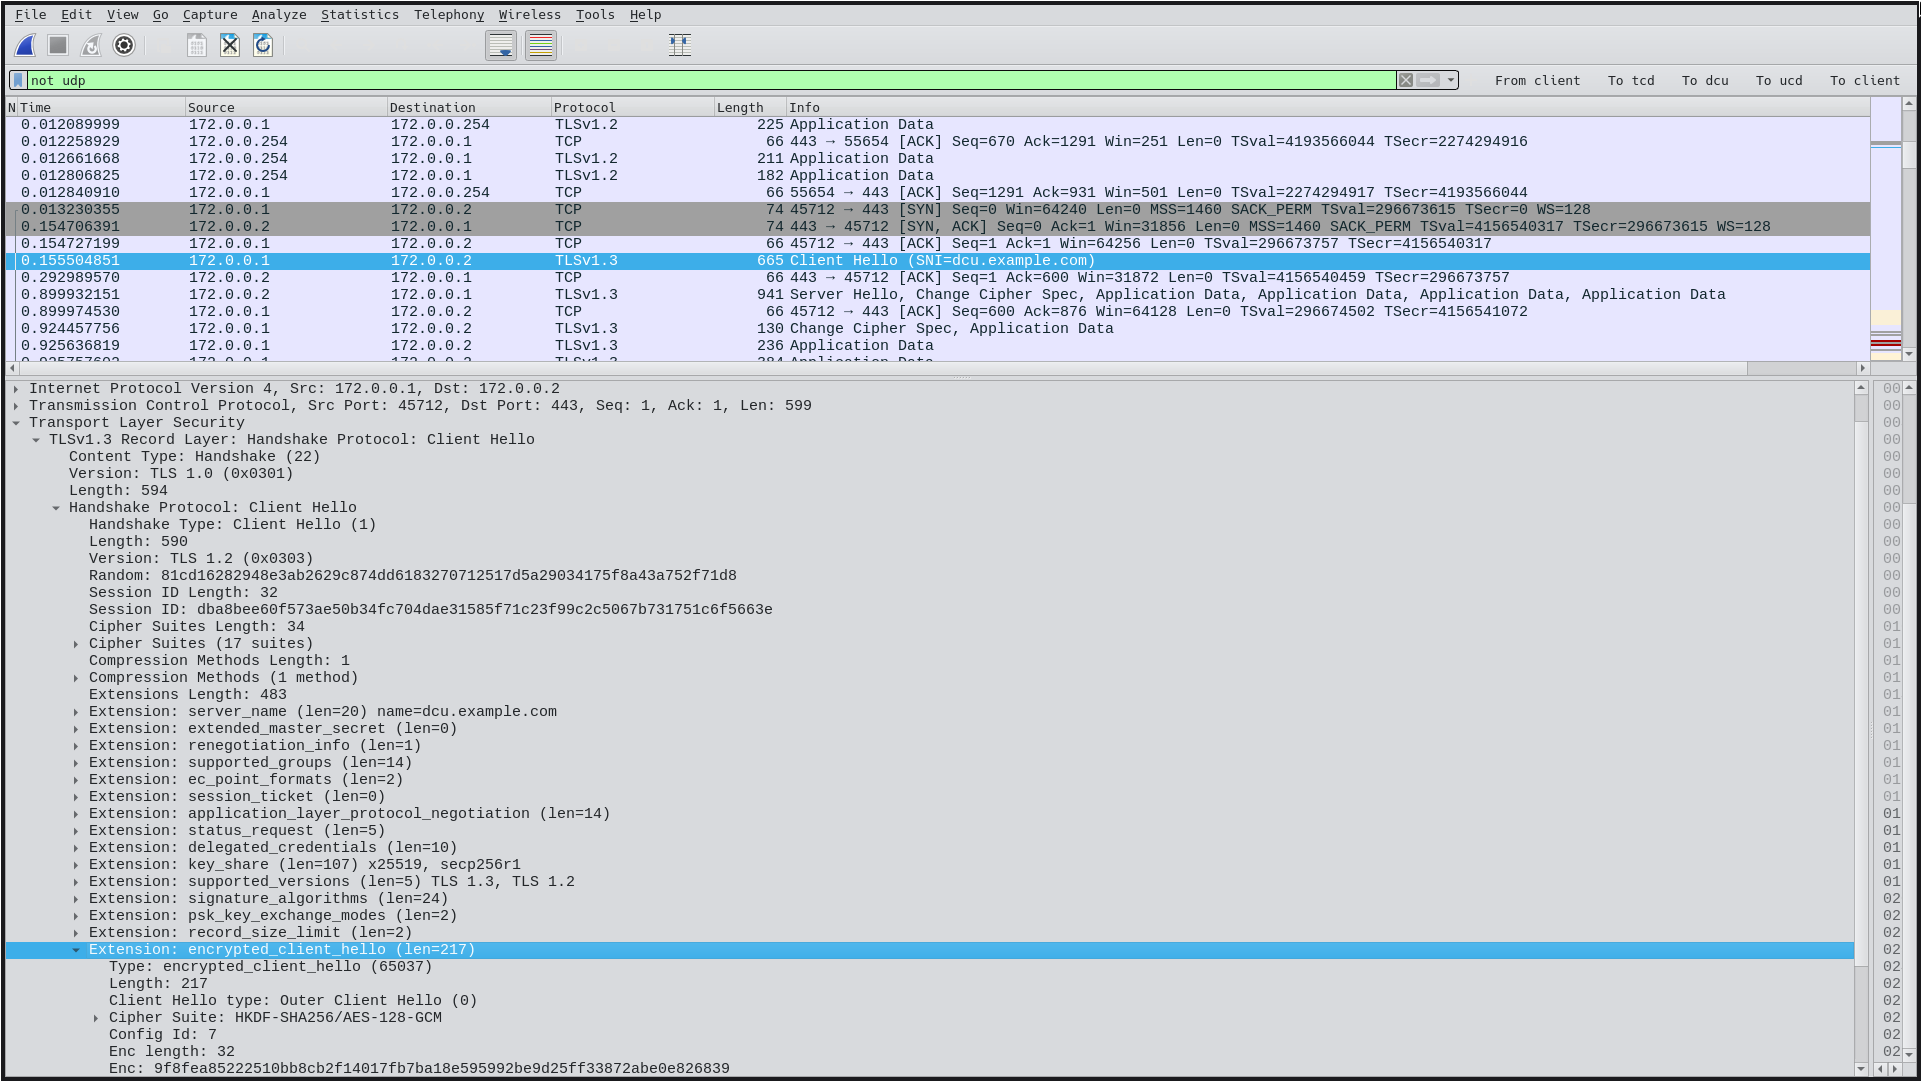
\includegraphics[width=120mm]{images/wireshark.png}}
\caption[TODO wireshark]{<>}
\label{wireshark_screenshot_figure}
\end{figure}









\section{Evaluation}

\blindtext

\subsection{Performance}

compare against normal ech and no ech
\blindtext

\begin{figure}[ht]
\centerline{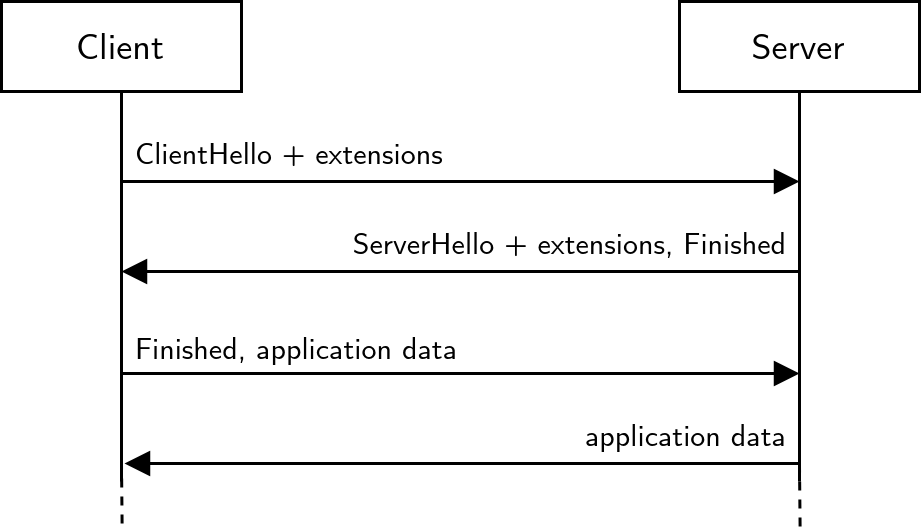
\includegraphics[width=120mm]{images/tls-handshake.png}}
\caption[TODO performance graph]{<latency vs >}
\label{performance_graph_figure}
\end{figure}

\subsection{Security}

\blindtext

\begin{figure}[ht]
\centerline{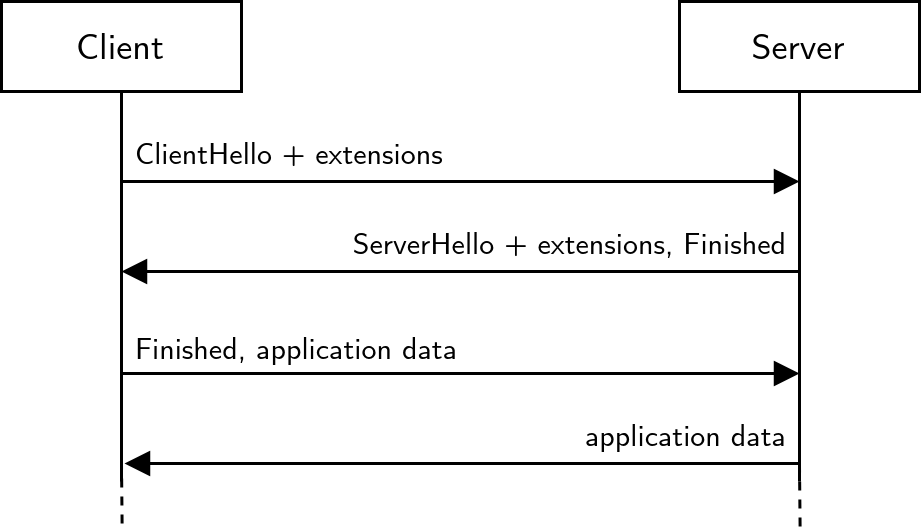
\includegraphics[width=120mm]{images/tls-handshake.png}}
\caption[TODO security graph using entropy or something]{<>}
\label{security_graph_figure}
\end{figure}








\section{Limitations}

\blindtext

\subsection{Load Balancing}

\blindtext

\subsection{Traffic Padding}

\blindtext









\section{Summary}

\blindtext
